% Tik output from JumanG
\documentclass[class=minimal,border=0pt]{article}
\usepackage{tikz}
\pagestyle{empty}
\usepackage{verbatim}
\begin{document}
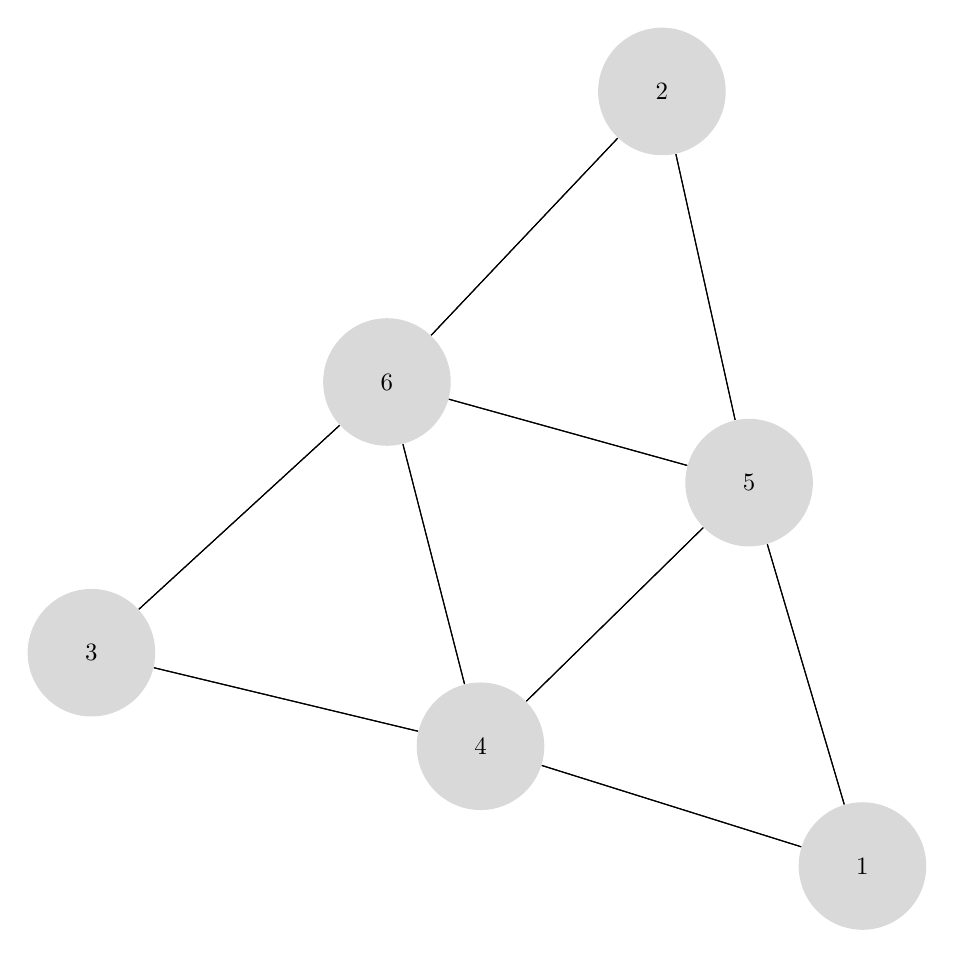
\begin{tikzpicture}[scale=0.90, transform shape]
	\tikzstyle{every node} = [circle, fill=gray!30, minimum size = 1.8cm]
	\node (1) at (4.55, -4.87) {1};
	\node (3) at (-6.33, -1.86) {3};
	\node (2) at (1.72, 6.06) {2};
	\node (5) at (2.95, 0.54) {5};
	\node (4) at (-0.84, -3.18) {4};
	\node (6) at (-2.16, 1.96) {6};
	\draw [-] (1)--(4);
	\draw [-] (1)--(5);
	\draw [-] (3)--(4);
	\draw [-] (3)--(6);
	\draw [-] (2)--(5);
	\draw [-] (2)--(6);
	\draw [-] (5)--(1);
	\draw [-] (5)--(2);
	\draw [-] (5)--(4);
	\draw [-] (5)--(6);
	\draw [-] (4)--(1);
	\draw [-] (4)--(3);
	\draw [-] (4)--(5);
	\draw [-] (4)--(6);
	\draw [-] (6)--(2);
	\draw [-] (6)--(3);
	\draw [-] (6)--(4);
	\draw [-] (6)--(5);
\end{tikzpicture}
\end{document}
